% vim: ts=4 sts=4 sw=4 et
\documentclass[nofonts, a4paper]{ctexart}

% 设置中文字体
\setCJKmainfont{AR PL UMing CN}
\setCJKsansfont{WenQuanYi Zen Hei}
\setCJKmonofont[Scale = 0.8]{AR PL UMing CN}

% 设置英文字体
\setmainfont{Liberation Serif}
\setsansfont{Droid Sans Mono}
\setmonofont{FreeMono}

\usepackage{amsmath}
\usepackage{amssymb}
\usepackage{graphics}
\usepackage{fancyhdr}
\usepackage{geometry}
\usepackage[font=small]{caption}
\usepackage{tikz}

% fancyhdr 风格设置
\pagestyle{fancy}   % 使用 fancy 风格 
\fancyhf{}          % 清除所有页眉页脚
\rhead{\thepage}    % 页号居页面右侧
\fancyhead[L]{\small{第七章\phantom{空}习题六}}

% 整体页面尺寸
\geometry{ left = 3cm, bottom = 2cm }

% 设置 section 格式
\CTEXsetup[number = {}, format = {\raggedright\bfseries\large}]{section}

% 标题信息
\title{第七章 \quad 分支限界算法}
\author{姓名: 吴周辉 \qquad 学号: 201428013229051}
\date{\today}

% 计数器
\newcounter{chapt}
\newcounter{subj}
\setcounter{chapt}{6}
\setcounter{subj}{0}

\begin{document}

\maketitle

\section{习题六}

\stepcounter{subj}
\thechapt.\thesubj 假设对旅行商问题的邻接矩阵如图1所示, 试用优先队列分枝
限界算法给出最短环游. 画出角空间的搜索树, 并说明搜索过程.

\begin{figure}[ht]
    \centering
    \begin{minipage}[c]{5cm}
        \[
            \begin{pmatrix}
                \infty	& 20		& 30		& 10		& 11		\\
                        & \infty	& 16		& 4			& 2			\\
 & 		& \infty	& 6			& 7			\\
                 &		&		& \infty	& 12		\\
                          &		&		&		& \infty	\\
            \end{pmatrix}
        \]
    \end{minipage}
    \begin{minipage}[c]{5cm}
        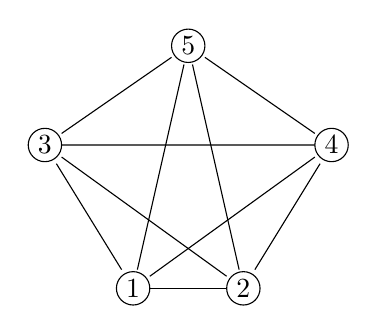
\begin{tikzpicture}[scale = 1.4]
            \node (A) at (1, 0){$1$};
            \node (B) at (2, 0){$2$};
            \node (C) at (0.2, 1.3){$3$};
            \node (D) at (2.8, 1.3){$4$};
            \node (E) at (1.5, 2.2){$5$};

            \draw (A) circle (1ex);
            \draw (B) circle (1ex);
            \draw (C) circle (1ex);
            \draw (D) circle (1ex);
            \draw (E) circle (1ex);

            \draw (A) -- (B);
            \draw (A) -- (C);
            \draw (A) -- (D);
            \draw (A) -- (E);
            \draw (B) -- (C);
            \draw (B) -- (D);
            \draw (B) -- (E);
            \draw (C) -- (D);
            \draw (C) -- (E);
            \draw (D) -- (E);
        \end{tikzpicture}
    \end{minipage}
    \caption*{图1}

\end{figure}

解: 解空间树如下图所示. 图中圆圈内的数字为结点的ID, 圆圈左边的数字是从
起点到该结点的路径长度, 叶子结点的路径长度还要加上到起点的距离. 圆圈右
边的数字是该结点被扩展的序号. 从下图可以看到, 问题的最优解为1-4-3-2-5%
-1, 1-4-3-5-2-1, 1-5-2-3-4-1, 路径长度均为45.
\begin{figure}
    \includegraphics[scale=0.15]{IMG_20141112_134805.jpg}
    \caption*{解6.1图}
\end{figure}

\stepcounter{subj}
\thechapt.\thesubj 最佳调度问题: 假设有 $n$ 个任务要由 $k$ 可并行工作
的机器完成, 完成任务需要的时间为 $t_i$. 试设计一个分枝限界算法, 找到
完成这 $n$个任务的最佳调度, 使得完成全部任务的时间最短.

解: 将这 $n$ 个任务按完成时间升序排列, 不妨设序列为 $1, 2, 3, \dots , n$,
满足 $ t_1 \le t_2 \le t_3 \le \dots \le t_n $, 将前 $k$ 个任务分别分配给 
$k$ 台机器, 每台机器一个任务, 将第 $k+1$ 个任务分配给当前最早完成任务的机
器, 再将 $k+2$ 个任务分配给当前最早完成任务的机器, 依此类推, 一直到第 $n$
个任务, 此时完成全部任务的时间记为 $T$, 将 $T$ 任务分枝限界函数, 在扩展
结点时, 如果当前的完成时间超过$T$, 则不必再往下扩展, 否则更新最优值.

如果机器完成所分配任务的时间越短, 则优先级越高, 选择优先级最高的节点作为
下一个扩展结点.

假设算法开始时, 已有 $k$ 个任务被分别分配到 $k$ 台机器上, 每次从堆 中选择
一个优先级最高的节点, 一直到堆空为止.
\linespread{0.8}
\begin{verbatim}
/* 解空间树的结点类型 */
struct Node {
    int path[n];    /* 解空间路径 */
    int time[k];    /* 每台机器上已分配的任务运行时间 */
    int time_all;   /* 到该结点为止的完成时间 */
    int depth;      /* 结点的深度 */
};

void best_sche(int n, int k, int t[])
{
    int best_time = n * max(t[]);
    root = new Node;

    root.path = {0...0};
    root.time = {0...0};
    root.time_all = 0;
    root.depth = 0;

    put2heap(heap, root);
    while (!heap.is_empty()) {
        next_node = pop(heap);

        for (i = 1; i <= k; i++) {
            x = new Node(next_node);
            x.depth++;
            x.path[x.depth] = i;
            x.time[i] += t[x.depth];
            x.time_all = max(x.time);

            if (x.depth == n) { /* 找到一个解 */
                if (x.time_all < best_time) {
                    best_time = x.time_all;
                    result      = x;
                }
            } else if (x.time_all < best_time) {
                put2heap(head, x);
            }
        }
    }
}
\end{verbatim}

\end{document}
